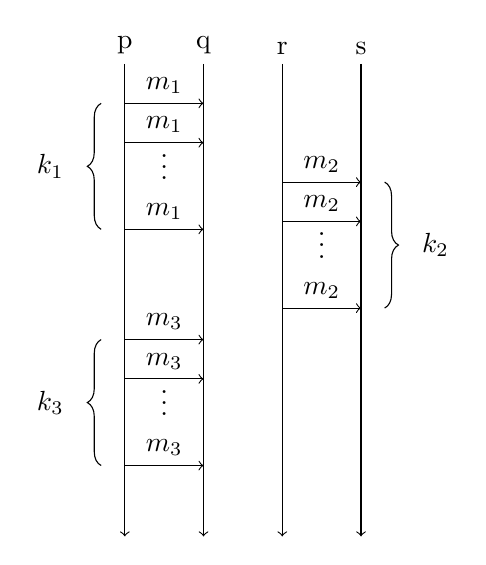
\begin{tikzpicture}
    \draw[->] (0,0) node [above] {p} -- (0,-6);
    \draw[->] (1,0) node [above] {q} -- (1,-6);
    \draw[->] (2,0) node [above] {r} -- (2,-6);
    \draw[->] (3,0) node [above] {s} -- (3,-6);

    \draw[->] (0,-.5) -- node [above] {$m_1$} (1,-.5);
    \draw[->] (0,-1) -- node [above] {$m_1$} (1,-1);
    \node at (.5,-1.2) {$\vdots$};
    \draw[->] (0,-2.1) -- node [above] {$m_1$} (1,-2.1);

    \draw[->] (2,-1.5) -- node [above] {$m_2$} (3,-1.5);
    \draw[->] (2,-2) -- node [above] {$m_2$} (3,-2);
    \node at (2.5,-2.2) {$\vdots$};
    \draw[->] (2,-3.1) -- node [above] {$m_2$} (3,-3.1);

    \draw[->] (0,-3.5) -- node [above] {$m_3$} (1,-3.5);
    \draw[->] (0,-4) -- node [above] {$m_3$} (1,-4);
    \node at (.5,-4.2) {$\vdots$};
    \draw[->] (0,-5.1) -- node [above] {$m_3$} (1,-5.1);

    % on ajoute des accolades
    \draw [decorate,decoration={brace,amplitude=5pt,mirror}] (-.3,-.5) -- node [midway, left=1em] {$k_1$} (-.3,-2.1) ;
    \draw [decorate,decoration={brace,amplitude=5pt,mirror}] (-.3,-3.5) -- node [midway, left=1em] {$k_3$} (-.3,-5.1) ;
    \draw [decorate,decoration={brace,amplitude=5pt}] (3.3,-1.5) -- node [midway, right=1em] {$k_2$} (3.3,-3.1) ;

\end{tikzpicture}
